\documentclass{article}
\usepackage{amsmath,amsthm,amssymb}
\usepackage{fontspec}
\usepackage{polyglossia}
\setdefaultlanguage{russian}
\setotherlanguage{english}
\setmainfont{DejaVu Serif}
\newfontfamily\cyrillicfont{DejaVu Serif}
\newfontfamily\cyrillicfontsf{DejaVu Sans}
\newfontfamily\cyrillicfonttt{DejaVu Sans Mono}
\usepackage{graphicx}
\usepackage{hyperref}

\graphicspath{{../artifacts/}}
\title{Определение токсичности комментариев}
\author{Екатерина Бойкова}
\date{2026}

\begin{document}
\maketitle

\begin{abstract}
В работе исследуется бинарная классификация токсичных англоязычных комментариев
Civil Comments. Исходный исследовательский прототип преобразован в воспроизводимый
эксперимент с независимым test-набором. Сравниваются частотный baseline,
логистическая регрессия, контролируемая абляция линейного SVM на словных
TF-IDF-признаках с символьными n-граммами и без них, а также дообученный
DistilBERT. Все модели
используют одинаковые splits; checkpoint и порог решения выбираются только на
validation. DistilBERT получил на test F1=0.637, PR-AUC=0.693 и ROC-AUC=0.938
против F1=0.554 у лучшего классического SVM. Код проекта:
\url{https://github.com/Ekotik15/Determining_the_toxicity_of_comments-}.
\end{abstract}

\section{Introduction}
Автоматическое обнаружение токсичности помогает модерировать большие
дискуссионные площадки. Задача сложна из-за дисбаланса классов, зависимости от
контекста, сарказма и субъективности разметки. False negative пропускает
вредоносный контент, а false positive может необоснованно ограничить нормальное
высказывание.

Цель проекта --- построить воспроизводимый классификатор, сравнить несколько
конкурентных подходов в одном протоколе и подготовить модель для
демонстрационного инференса. Текст комментария отображается в бинарную метку
$y \in \{0, 1\}$, где 1 означает токсичный комментарий.

Отличия итогового подхода от исходного прототипа: независимый test не
используется при выборе модели или порога; все подходы оцениваются одинаковыми
метриками; дисбаланс учитывается весами классов без SMOTE; Streamlit
демонстрирует сохранённую классическую SVM с её validation-порогом, а DistilBERT
сравнивается в том же протоколе и запускается отдельно; артефакты сохраняются
автоматически.

\subsection{Team}
\textbf{Екатерина Бойкова} выполнила постановку задачи, исследование данных,
разработку и сравнение моделей, анализ результатов и подготовку
демонстрационного приложения.

\section{Related Work}
\label{sec:related}
Линейные модели на TF-IDF остаются важными baseline для классификации текста:
они быстры, интерпретируемы и эффективны при ограниченных вычислительных
ресурсах. Символьные n-граммы устойчивы к опечаткам, вариантам написания и
намеренной обфускации.

Duchêne et al.~\cite{duchene2023benchmark} сравнили CNN, RNN, BERT, DistilBERT,
RoBERTa, XLNet и другие архитектуры на Civil Comments. RoBERTa с focal loss
показывает сильное качество и устойчивость к смещению, а DistilBERT обеспечивает
компромисс между AUROC и временем инференса. Их многометочный протокол отличается
от текущей бинарной постановки.

Borkan et al.~\cite{borkan2019nuanced} предложили subgroup AUC, BPSN AUC и BNSP
AUC для измерения unintended bias. Vaidya et al.~\cite{vaidya2019empirical}
исследовали multi-task learning с совместным предсказанием токсичности и
идентичностей. Reichert et al.~\cite{reichert2020reading} сравнили балансировку,
TF-IDF, GloVe, нейронные сети и LSTM. Nanda et
al.~\cite{nanda2021empirical} показали, что лучший подход по AUC не обязательно
является лучшим по всем fairness-метрикам.

Текущая работа не претендует на state of the art, но содержит прямое
same-protocol сравнение классических моделей с современным Transformer-baseline.

В таблице~\ref{tab:previous-art} приведены выбранные результаты Duch\^ene et
al.~\cite{duchene2023benchmark}. Они получены в многометочной постановке примерно
на 310 тыс. обучающих примеров и поэтому не сопоставляются напрямую с текущим
бинарным протоколом.

\begin{table}[tbh!]
\centering
\small
\begin{tabular}{|l|l|r|r|r|}
\hline
Model & Protocol & AUROC & Macro-F1 & Recall\\
\hline
DistilBERT & multilabel & 0.9804 & 0.3879 & 0.9001\\
RoBERTa BCE & multilabel & 0.9813 & 0.4749 & 0.8891\\
RoBERTa focal loss & multilabel & 0.9818 & 0.4648 & 0.8839\\
BiLSTM & multilabel & 0.9754 & 0.3638 & 0.8761\\
\hline
\end{tabular}
\caption{Выбранные результаты previous art; протокол отличается от текущей работы.}
\label{tab:previous-art}
\end{table}

\section{Model Description}
Итоговый кандидат объединяет словные и символьные TF-IDF-признаки. Словный
векторизатор использует униграммы и биграммы, \texttt{min\_df=2},
\texttt{max\_df=0.995}, sublinear TF и до 40\,000 признаков. Символьный
векторизатор использует \texttt{char\_wb} n-граммы длины 3--5,
\texttt{min\_df=3} и до 40\,000 признаков.

Для текста $d$ и терма $t$ используется вес
\[
\operatorname{TFIDF}(t,d)=\operatorname{TF}(t,d)
\log\frac{N}{\operatorname{DF}(t)},
\]
где $N$ --- число документов, а $\operatorname{DF}(t)$ --- число документов,
содержащих терм. Sublinear TF заменяет частоту на $1+\log(\operatorname{TF})$.

Объединённый разреженный вектор подаётся в LinearSVC с $C=1.5$ и
\texttt{class\_weight=balanced}. Decision scores калибруются sigmoid-методом на
трёх фолдах. Порог выбирается на validation по максимуму F1 положительного
класса. SMOTE исключён, поскольку интерполяция разреженных TF-IDF-векторов не
соответствует реальным текстам.

\subsection{Transformer baseline}
Используется \texttt{distilbert-base-uncased}~\cite{sanh2019distilbert} с
классификационной головой на два класса. Вес токсичного класса равен отношению
числа отрицательных примеров к положительным. Лучший checkpoint и decision
threshold выбираются на validation, после чего фиксированная конфигурация один
раз оценивается на test. CUDA и mixed precision включаются автоматически при
наличии GPU; локальный полный запуск выполнен на CPU в сокращённой одноэпоховой
конфигурации.

\section{Dataset}
Используется \texttt{mteb/toxic\_conversations\_50k}~\cite{mtebdataset},
созданный на основе Jigsaw Unintended Bias in Toxicity
Classification~\cite{jigsaw2019unintended} и архива
Civil Comments. Комментарии опубликованы на англоязычных новостных площадках в
2015--2017 годах. Лицензия набора --- CC BY 4.0. Данные доступны по адресу
\url{https://huggingface.co/datasets/mteb/toxic_conversations_50k}.

Токсичность оценивали десять аннотаторов. Бинарная метка соответствует порогу
\texttt{target >= 0.5}. Исходно доступны 50\,000 train- и 50\,000 test-строк.
Удаляются пустые тексты, дубликаты и пересечения train с test. Очищенный train
делится стратифицированно: 80\% для обучения и 20\% для validation.

\begin{table}[tbh!]
\centering
\begin{tabular}{|l|r|r|r|r|}
\hline
Split & Rows & Toxic & Toxic share & Median chars\\
\hline
Train & 39\,832 & 3\,166 & 7.95\% & 204\\
Validation & 9\,958 & 791 & 7.94\% & 209\\
Test & 49\,896 & 3\,947 & 7.91\% & 202\\
\hline
\end{tabular}
\caption{Статистика данных после очистки и разбиения.}
\label{tab:dataset}
\end{table}

Положительный класс составляет около 8\%, поэтому accuracy сама по себе
неинформативна.

Карточка набора указывает на дополнительную обработку в MTEB/MMTEB; поэтому для
происхождения данных также учитываются описания MTEB~\cite{muennighoff2023mteb}
и MMTEB~\cite{enevoldsen2025mmteb}. Использованная conversion revision
\nolinkurl{ab3aee44e1d13d6938102bef4c6af909e6a9799d} зафиксирована вместе с
SHA-256: train ---
\nolinkurl{d27d62973dfc05d1931c5cde813a65792c960cae4e1de914b7650f2c8d00376a},
test ---
\nolinkurl{0da0742843c8c94406779a18d6a9c575e4a592e7e650fee52593e9cf5c9475cd}.
Эти файлы содержат по 50\,000 исходных строк. Текущая metadata карточки описывает
canonical test split из 2\,048 строк, то есть другой вариант публикации; все
результаты ниже относятся только к зафиксированным Parquet-файлам.

\section{Experiments}
\subsection{Metrics}
Основной критерий выбора --- F1 токсичного класса:
\[
F_1 = 2\frac{\mathrm{Precision}\cdot\mathrm{Recall}}
{\mathrm{Precision}+\mathrm{Recall}}.
\]
Дополнительно рассчитываются macro-F1, PR-AUC, ROC-AUC и accuracy. PR-AUC
особенно важен при редком положительном классе.

\subsection{Experiment Setup}
Эксперимент выполняется с \texttt{random\_state=42} на Python 3.10.
Используются scikit-learn 1.7.2, pandas 2.3.3, NumPy 2.2.6, PyArrow 24.0.0,
PyTorch 2.8.0 и Transformers 4.56.2.
Выполняется один детерминированный запуск. Каждая модель обучается на одном
train. Порог выбирается только на validation, после чего фиксированные модель и
порог один раз оцениваются на test. Победитель определяется по validation F1.
Опубликованный Transformer-запуск использует одну эпоху, максимальную длину
128 tokens, train batch size 16, eval batch size 64, learning rate $2\cdot10^{-5}$,
weight decay 0.01 и random state 42; точная CLI-команда приведена в README.

Для итоговой модели дополнительно рассчитываются 95\% интервалы методом
стратифицированного непараметрического bootstrap фиксированных test-предсказаний
(1000 повторов, random state 42). Эти интервалы отражают вариативность test,
но не вариативность повторного обучения.

\subsection{Baselines}
Сравниваются:
\begin{itemize}
\item Dummy prior --- нижняя граница, использующая только частоты классов;
\item word TF-IDF + Logistic Regression с $C=4.0$,
\texttt{class\_weight=balanced} и \texttt{solver=liblinear};
\item word TF-IDF + calibrated Linear SVM;
\item word+character TF-IDF + calibrated Linear SVM --- основной классический подход;
\item fine-tuned \texttt{distilbert-base-uncased} со взвешенной cross-entropy.
\end{itemize}
Две SVM-конфигурации отличаются только набором признаков: $C=1.5$, веса классов,
трёхфолдовая sigmoid-калибровка, splits и выбор порога остаются неизменными.

\section{Results}
\begin{table}[tbh!]
\centering
\resizebox{\linewidth}{!}{
\begin{tabular}{|l|l|rrrrrr|}
\hline
Model & Split & Precision & Recall & F1 & Macro-F1 & PR-AUC & ROC-AUC\\
\hline
Dummy prior & validation & 0.000 & 0.000 & 0.000 & 0.479 & 0.079 & 0.500\\
Dummy prior & test & 0.000 & 0.000 & 0.000 & 0.479 & 0.079 & 0.500\\
Logistic Regression & validation & 0.569 & 0.537 & 0.553 & 0.758 & 0.556 & 0.875\\
Logistic Regression & test & 0.550 & 0.513 & 0.531 & 0.746 & 0.552 & 0.879\\
Word SVM & validation & 0.588 & 0.504 & 0.543 & 0.753 & 0.548 & 0.867\\
Word SVM & test & 0.562 & 0.485 & 0.521 & 0.741 & 0.547 & 0.872\\
Word+char SVM & validation & 0.577 & 0.549 & 0.563 & 0.763 & 0.591 & 0.892\\
Word+char SVM & test & 0.559 & 0.550 & 0.554 & 0.758 & 0.594 & 0.895\\
DistilBERT & validation & 0.630 & 0.626 & 0.628 & 0.798 & 0.680 & 0.932\\
DistilBERT & test & 0.625 & 0.649 & 0.637 & 0.802 & 0.693 & 0.938\\
\hline
\end{tabular}}
\caption{Результаты всех подходов.}
\label{tab:results}
\end{table}

По validation выбран DistilBERT с порогом 0.622. На независимом test он получил
F1=0.637, macro-F1=0.802, PR-AUC=0.693 и ROC-AUC=0.938. Прирост F1 относительно
лучшего классического SVM равен 0.082. Accuracy dummy-модели превышает 92\%, хотя
она не обнаруживает ни одного токсичного комментария, что подтверждает
необходимость F1 и PR-AUC.

В контролируемой абляции добавление символьных n-грамм повышает test F1 с
0.521 до 0.554 ($+0.034$), а PR-AUC --- с 0.547 до 0.594 ($+0.047$).
Поскольку классификатор и протокол одинаковы, различие можно связать именно с
добавлением character-признаков в рамках данного запуска.

\begin{table}[tbh!]
\centering
\small
\begin{tabular}{|l|r|r|r|r|r|}
\hline
Threshold policy & Threshold & Accuracy & Precision & Recall & F1\\
\hline
Default & 0.500 & 0.937 & 0.590 & 0.674 & 0.629\\
Validation-selected & 0.622 & 0.941 & 0.625 & 0.649 & 0.637\\
\hline
\end{tabular}
\caption{Влияние порога на test-метрики итоговой модели.}
\label{tab:threshold}
\end{table}

Validation-selected threshold повышает precision и F1 ценой небольшого снижения
recall. Порог настраивается только на validation, а не по test.

\begin{table}[tbh!]
\centering
\small
\begin{tabular}{|l|r|r|r|}
\hline
Metric & Estimate & 95\% CI lower & 95\% CI upper\\
\hline
Precision & 0.625 & 0.612 & 0.637\\
Recall & 0.649 & 0.634 & 0.663\\
F1 toxic & 0.637 & 0.625 & 0.649\\
PR-AUC & 0.693 & 0.679 & 0.706\\
ROC-AUC & 0.938 & 0.933 & 0.941\\
\hline
\end{tabular}
\caption{Bootstrap-интервалы итоговых test-метрик.}
\label{tab:ci}
\end{table}

\begin{figure}[tbh!]
\centering
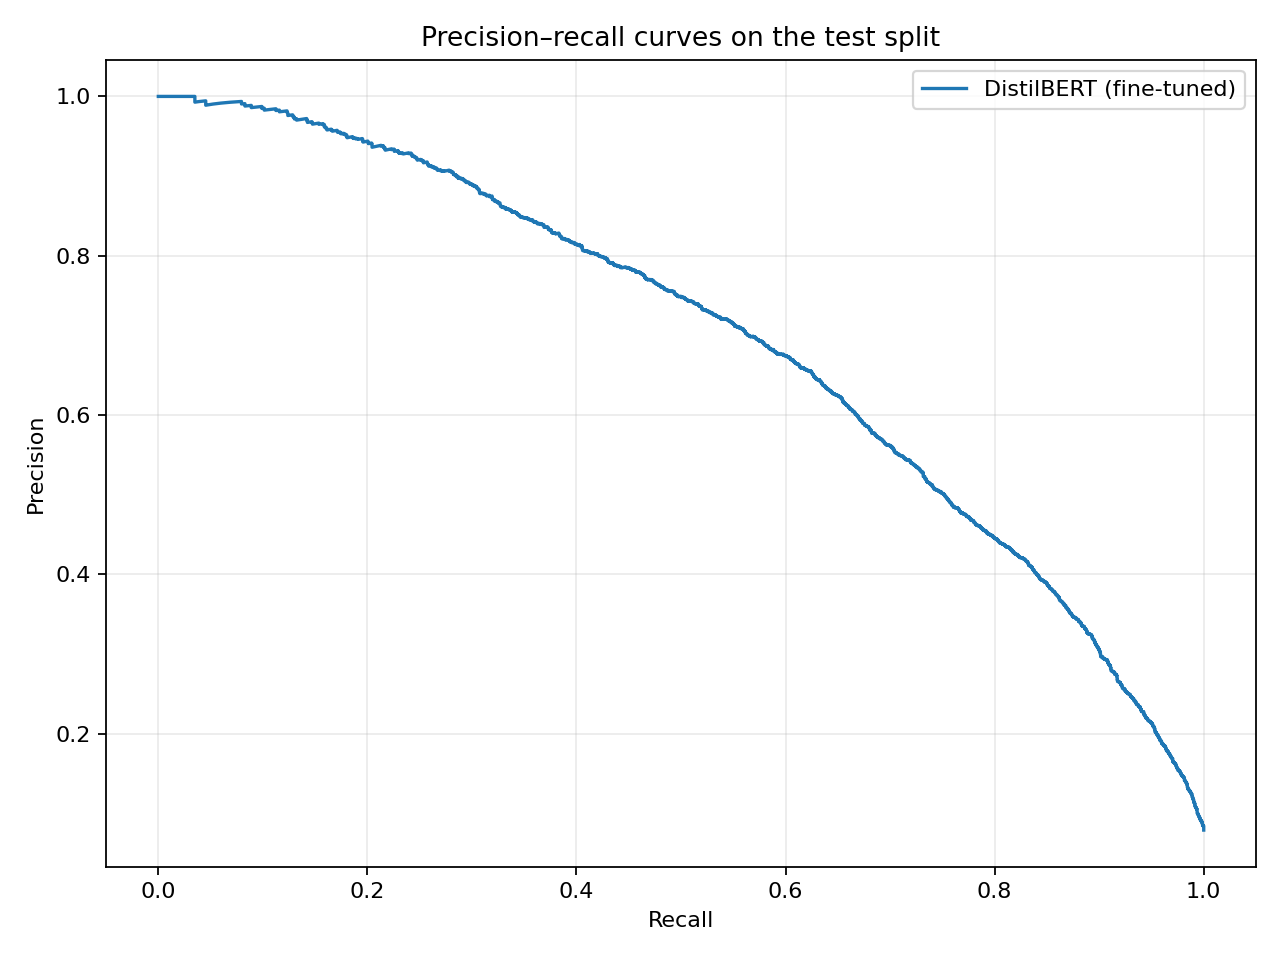
\includegraphics[width=0.72\linewidth]{precision_recall_curves.png}
\caption{Precision--recall curves на независимом test.}
\label{fig:pr}
\end{figure}

\begin{figure}[tbh!]
\centering
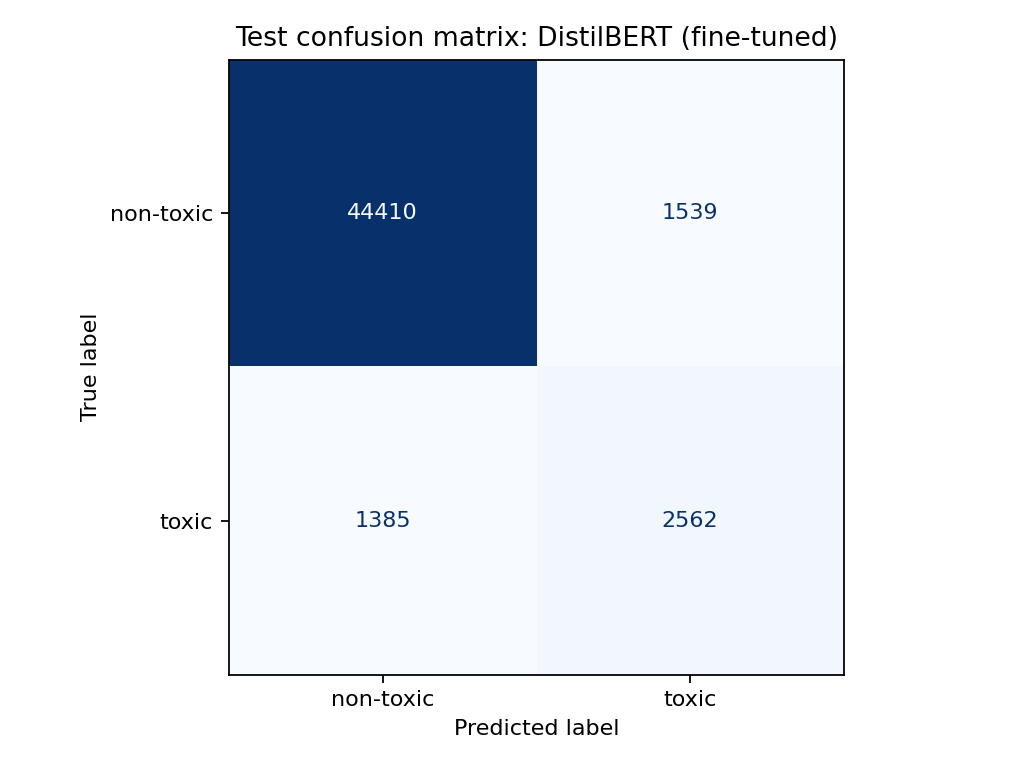
\includegraphics[width=0.62\linewidth]{confusion_matrix.png}
\caption{Confusion matrix выбранной модели на test.}
\label{fig:cm}
\end{figure}

Матрица ошибок содержит 44,410 true negative, 1,539 false positive, 1,385 false
negative и 2,562 true positive. False positive rate равен 3.35\%, а false
negative rate --- 35.09\%. Высоко уверенные false positive часто содержат
отдельные оскорбительные слова вне прямой атаки, а false negative выражают
токсичность через контекст, иронию или редкие формулировки. Некоторые случаи
указывают на возможный шум бинарной разметки.

\section{Conclusion}
Исследовательский ноутбук преобразован в воспроизводимый проект: реализованы
независимый test, фиксированный validation-протокол, конкурентные baseline,
сохранение артефактов, unit-тесты и демонстрационный Streamlit-инференс
классической модели. DistilBERT дообучен и напрямую сравнен с классическими
подходами на тех же splits.

Работа не заявляет SotA, поскольку опубликованные исследования используют другие
подвыборки, labels или fairness-протоколы. Ограничения включают англоязычный
домен 2015--2017 годов, субъективность разметки и identity bias. Модель нельзя
использовать как единственный источник решения о блокировке; безопасный сценарий
--- ранжирование для ручной модерации.

Контролируемая абляция подтверждает пользу символьных n-грамм для выбранного
линейного SVM: test F1 вырос на 0.034 при неизменных классификаторе, калибровке,
splits и процедуре выбора порога.

Дальнейшая работа: повторить Transformer-обучение на GPU для нескольких seed,
сравнить DistilBERT с RoBERTa, добавить subgroup/BPSN/BNSP AUC и измерить
стоимость инференса.

\bibliographystyle{plain}
\bibliography{lit}
\end{document}
